\documentclass[a4paper, 12pt]{article}

\usepackage{cmap} % поиск в PDF l
\usepackage[T2A]{fontenc} % кодировка

\usepackage[utf8]{inputenc} % кодировка исходного текста
\usepackage[english,russian]{babel} % локализация и переносы
\usepackage{amsmath, amsfonts, amssymb, amsthm, mathtools, float}
\usepackage{ stmaryrd }

% Рисунки
\usepackage{graphicx}
\usepackage{wrapfig}

\usepackage[left=2cm,right=2cm, top=2cm,bottom=2cm,bindingoffset=0cm]{geometry}

\usepackage{longtable}

\graphicspath{pictures}

\author{Балдин Виктор}
\title{Работа 1.2.4 \\ Определение главных моментов инерции твердых тел с помощью крутильных колебаний}

\begin{document}

	\maketitle
	\section{Аннотация}
	\textbf{Цель работы:} измерить периоды крутильных колебаний рамки при различных положениях закрепленного
	в ней тела, проверить теоретическую зависимость между периодами крутильных колебаний тела
	относительно различных осей, определить моменты инерции относительно нескольких осей для каждого тела,
	по ним найти главные моменты инерции тела и построить эллипсоид инерции.
	\bigskip\\
	\textbf{Оборудование:} установка для получения крутильных колебаний, набор исследуемых твердых тел, секундомер.

	\section{Теоретические сведения}
	Инерционные свойства твердого тела при вращении определяется
	 пространственным распределением. Оно характеризуется тензором инерции тела. Тензор инерции твердого тела
	 является симметричным тензором 2-ого ранга $J\in  T_{2}^{0}(V)$ и имеет 6 независимых компонент,
	 которые в прямоугольной декартовой системе координат выражаются как:
	\begin{equation}
	    I_{ij}=\int (\delta _{ij}r^{2}-r_{i}r_{j}) \ dm =I_{ji},
	\end{equation}
	 где $r$ — расстояния от точек до центра, относительно которого вычисляется тензор инерции,
	а $r_{i}$ — координатные компоненты соответствующих отрезков, $i$ и $j$ — номера координат (от 1 до 3).\\
	Если для какой либо системы координат все 6 компонент известны, то момент инерции тела относительно
	 произвольной оси $l$, проходящей через начало координат может быть вычислен по формуле:
	\begin{equation}
	    I_{l}=n^{j}n^{i}I_{ij}=\vec{n}^{T} I \vec{n}
	\end{equation}
	где $\vec{n}$ - единичный вектор-столбец который задает направление оси, $I$ - тензор инерции.\\
	А момент импульса $\vec  {L}$ и вращательная энергия тела $E_{\text{вращ}}$ тогда будут выражаться как:
	\begin{equation}
	    E_{\text{вращ}}={1 \over 2}\ {\vec {\omega }}^{\,T} I {\vec {\omega }} ={1 \over 2}\sum _{{ij}}\omega^{i}J_{{ij}}\omega^{j}
	\end{equation}
	\begin{equation}
	    {\vec  {L}}=I {\vec  {\omega }}, \ \ \ \ L_{i}=\sum _{j}I_{{ij}}\omega^{j}
	\end{equation}
	Отложим вдоль оси $l$ из начала координат радиус-вектор $r$
	равный по длине $1/\sqrt{I_{l}}$. Проведем множество таких отрезков, соответствующих различным направлениям оси $l$.
	 Геометрическое место концов указанных отрезков, является поверхность второго порядка - эллипсоид. Этот эллипсоид принято называть
	 эллипсоидом инерции. Он жестко связан с телом для которого он построен. Знание эллипсоида инерции позволяет найти момент инерции тела
	относительно любой оси, проходящей через центр эллипсоида. Длина отрезка $r$ будет определять момент инерции тела относительно оси $l$:
	\begin{equation}
	    I_{l} = \frac{1}{r^2}
	\end{equation}
	\begin{figure}[H]
		\centering
		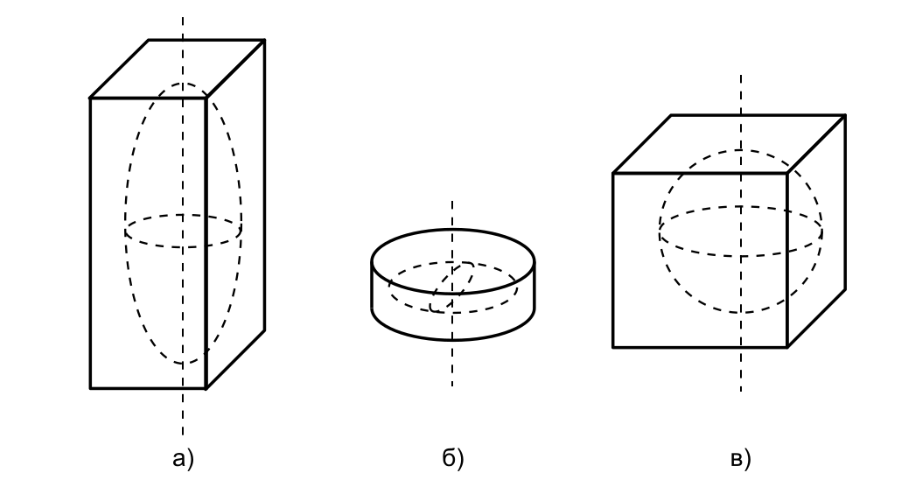
\includegraphics[scale = 0.5]{pictures/ellipsoid.png}
		\caption{Эллипсоиды вращения для разных тел}
	\end{figure}

	Как и всякий симметричный тензор второго ранга может быть диагонализован некоторой заменой координат.
	Пусть система координат, в которой он диагонализован имеет оси $Ox,Oy,Oz$, тогда эти оси совпадают с главными осями тела.
	Полученные диагональные элементы $I_{x}, I_{y}, I_{z}$ называются главными моментами инерции тела, а уравнение эллипсоида
	 инерции в этих координатах примет вид:
	\begin{equation}
	    I_{x}r^{2}_{x}+I_{y}r^{2}_{y}+I_{z}r^{2}_{z} = 1
	\end{equation}
	Крутильные колебания рамки с телом описываются уравнением:
	\begin{equation}
	    (I + I_p)\ddot{\varphi} + f \varphi = 0
	\end{equation}
	Здесь $I$ и $I_{p}$ - моменты инерции тела и рамки относительно
	 оси вращения, $\varphi$ - угол поворота рамки, меняющийся со
	временем $t$, $f$ - модуль кручения проволоки. Отсюда период этих колебаний:
	\begin{equation}
	    T = 2\pi\sqrt{\frac{I+I_{p}}{f}}
	\end{equation}
	На рисунке показано, как проходят оси вращения в параллелепипеде.
	 Оси $AA'$, $BB'$ и $CC'$ являются главными. Моменты инерции относительно
	этих осей обозначим соответственно $I_{x}, I_{y}, I_{z}$.\\

	\begin{figure}[H]
	    \begin{center}
	        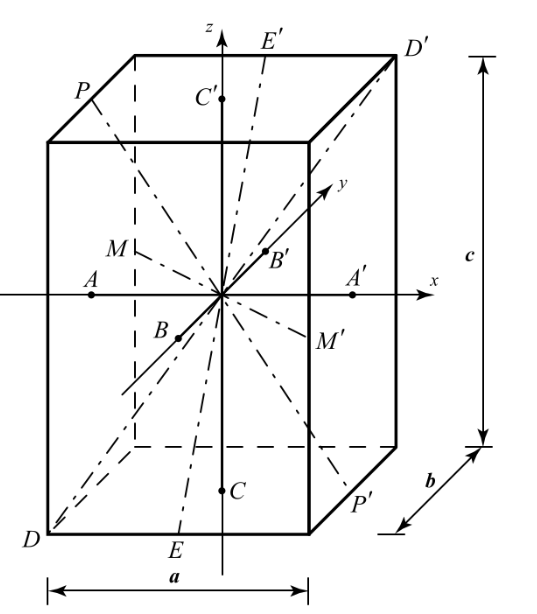
\includegraphics[scale=0.5]{pictures/kyb.png}
	        \caption{Оси вращения прямоугольного параллелепипеда}
	        \label{graphic1}
	    \end{center}
	\end{figure}

	Момент инерции $I_{D}$ при вращении относительно диагонали $DD'$ выражается
	 через главные моменты с помощью формулы:
	\begin{equation}
	    I_{d}=I_{x}\frac{a^2}{d^2}+I_{y}\frac{b^2}{d^2}+I_{z}\frac{c^2}{d^2}
	\end{equation}
	Используя связь момента инерции с периодом крутильных колебаний
	получаем соотношение между периодами колебаний относительно осей $DD'$, $EE'$,
	$MM'$ и $PP'$ с периодами крутильных колебаний относительно главных осей.
	\begin{equation}
		\begin{cases}
		(b^2+c^2)T^2_{E}=b^2 T^2_{y}+c^2 T^2_{z} \\
		(a^2+c^2)T^2_{P}=a^2 T^2_{x}+c^2 T^2_{z} \\
		(a^2+b^2)T^2_{M}=a^2 T^2_{x}+b^2 T^2_{y}
		\end{cases}
	\end{equation}

	Эти соотношения также необходимо проверить экспериментально.

 	\section{Методика измерений}
	В данной работе используется установка для измерения крутильных колебаний, приведенная
	на рисунке 3. Рамка 1 жестко соединена с проволокой 2, закрепленной вертикально в специальных
	зажимах 3, позволяющих сообщить начальное закручивание для возбуждения крутильных колебаний
	вокруг вертикальной оси.
	\begin{figure}[H]
		\centering
		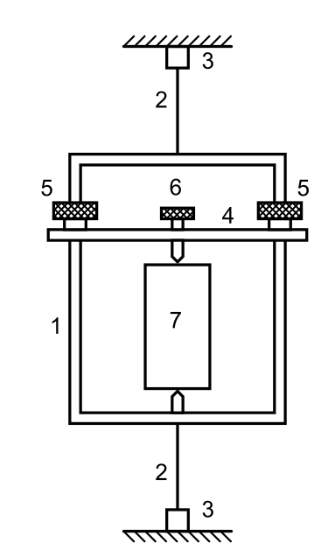
\includegraphics[scale = 0.5]{pictures/stand.png}
		\caption{Схема установки}
	\end{figure}

%
%
	\section{Используемое оборудование}
	Установка для получения крутильных колебаний, набор исследуемых твердых тел, секундомер.

%
	\section{Результаты измерений и обработка данных}
	\begin{enumerate}
		\item Измерим период сначала для ненагруженной рамки (здесь и далее
		период измеряем $N = 15$ раз, погрешность секундомера считаем приблизительно
		равной $\sigma_t^{\text{ сист }} = 0.20$ с):
		\begin{table}[H]
			\centering
			\caption{Колебания рамки}
			\begin{tabular}{|c|c|c|c|c|c|}
			\hline
			$t$, c & 38.4 & 38.6 & 38.6 & 38.6 & 38.5 \\ \hline
			$T$, c & 2.56 & 2.57 & 2.57 & 2.57 & 2.57 \\ \hline
			\end{tabular}
		\end{table}

		Отсюда средний период
		$$ \overline {T}_{p} = \frac{1}{N}\sum_{i} T_i = 2.57\; \text{с}, $$
		Среднеквадратичное отклонение
		$$ \sigma_T^{\text{ случ }} = \sqrt{\frac{ \sum_{i} (T_i - \overline {T})^2}{N} } = 0.01\; \text{с} $$
	%
		Общая погрешность таким образом равна:
		$$ \sigma_T = \frac{\sigma_t^{\text{ сист }}}{N} + \sigma_T^{\text{ случ }} = 0.03\; \text{с}$$

		\item Измерим размеры и массу цилиндра:
		\begin{table}[H]
			\centering
			\caption{Измерения размеров цилиндра}
			\begin{tabular}{|c|c|c|c|c|c|c|c|c|c|c|c|c|}
			\hline
			№       & 1    & 2    & 3    & 4    & 5    & 6    & 7    & 8    & 9    & 10   & Среднее & $\sigma$ \\ \hline
			$h$, мм & 49.1 & 49.5 & 49.3 & 49.3 & 49.2 & 49.2 & 49.2 & 49.4 & 49.2 & 49.2 & 49.3    & 0.2                    \\ \hline
			$d$, мм & 88.3 & 88.1 & 88.1 & 88.1 & 88.1 & 88.1 & 88.1 & 88.1 & 88.1 & 88.0 & 88.1    & 0.2                    \\ \hline
			\end{tabular}
		\end{table}

		Масса $m_{\text{цил}} = 2.264\pm0.001$ кг.
		Отсюда момент инерции
		$$I_{\text{цил}} = \frac{1}{8}md^2 = 2197\; \text{кг} \cdot \text{мм} ^2, $$
		$$ \sigma_I = I\sqrt{\left( \frac{\sigma_m}{m} \right) ^ 2 + 2\left( \frac{\sigma_d}
		{\overline{d}} \right) ^ 2} = 8\; \text{кг} \cdot \text{мм} ^2 $$

		\item Измерим период колебаний цилиндра
		\begin{table}[H]
			\centering
			\caption{Колебания цилиндра}
			\begin{tabular}{|cccccc|}
			\hline
			\multicolumn{6}{|c|}{Главная ось}                                                                                                                   \\ \hline
			\multicolumn{1}{|c|}{$t$, c} & \multicolumn{1}{c|}{47.9} & \multicolumn{1}{c|}{47.6} & \multicolumn{1}{c|}{47.2} & \multicolumn{1}{c|}{47.4} & 47.6 \\ \hline
			\multicolumn{1}{|c|}{$T$, c} & \multicolumn{1}{c|}{3.19} & \multicolumn{1}{c|}{3.17} & \multicolumn{1}{c|}{3.15} & \multicolumn{1}{c|}{3.16} & 3.17 \\ \hline
			\multicolumn{6}{|c|}{Боковая ось}                                                                                                                   \\ \hline
			\multicolumn{1}{|c|}{$t$, c} & \multicolumn{1}{c|}{45.1} & \multicolumn{1}{c|}{45.0} & \multicolumn{1}{c|}{45.3} & \multicolumn{1}{c|}{45.0} & 44.9 \\ \hline
			\multicolumn{1}{|c|}{$T$, c} & \multicolumn{1}{c|}{3.01} & \multicolumn{1}{c|}{3.00} & \multicolumn{1}{c|}{3.02} & \multicolumn{1}{c|}{3.00} & 2.99 \\ \hline
			\end{tabular}
		\end{table}

		$$ \overline{T}_{z}^{\text{цил}} = 3.17 \; \text{с}, \\\ \overline{T}_{x}^{\text{цил}} = 3.00\; \text{с} $$

		\item Найдем момент инерции рамки через формулу (8):
		$$ \frac{T_p}{T_{z}^{\text{цил}}} = \sqrt{\frac{I_p}{I_p + I_{\text{цил}}}}, $$
		$$ I_p = I_{\text{цил}} \frac{T_p^2}{(T_z^{\text{цил}})^2 - T_p^2} = 4213\; \text{кг} \cdot \text{мм} ^2 $$
		$$ \varepsilon_{I_p} = \frac{\sigma_I}{I} + 4\varepsilon_T = 0.06 $$

		\item Повторим все те же действия теперь для куба:
		\begin{table}[H]
			\centering
			\caption{Измерения для куба}
			\begin{tabular}{|ccccccccccccc|}
			\hline
			\multicolumn{13}{|c|}{Измерения длины}                                                                                                                                                                                                                                                                                                                                        \\ \hline
			\multicolumn{1}{|c|}{№}       & \multicolumn{1}{c|}{1}    & \multicolumn{1}{c|}{2}    & \multicolumn{1}{c|}{3}    & \multicolumn{1}{c|}{4}    & \multicolumn{1}{c|}{5}    & \multicolumn{1}{c|}{6}       & \multicolumn{1}{c|}{7}    & \multicolumn{1}{c|}{8}    & \multicolumn{1}{c|}{9}    & \multicolumn{1}{c|}{10}   & \multicolumn{1}{c|}{$\overline{a}$} & $\sigma_{a}$ \\ \hline
			\multicolumn{1}{|c|}{$a$, мм} & \multicolumn{1}{c|}{92.7} & \multicolumn{1}{c|}{92.8} & \multicolumn{1}{c|}{92.8} & \multicolumn{1}{c|}{92.6} & \multicolumn{1}{c|}{92.6} & \multicolumn{1}{c|}{92.6}    & \multicolumn{1}{c|}{92.6} & \multicolumn{1}{c|}{92.6} & \multicolumn{1}{c|}{92.7} & \multicolumn{1}{c|}{92.8} & \multicolumn{1}{c|}{92.7}           & 0.1          \\ \hline
			\multicolumn{13}{|c|}{Ось $AA’$}                                                                                                                                                                                                                                                                                                                                              \\ \hline
			\multicolumn{1}{|c|}{№}       & \multicolumn{1}{c|}{1}    & \multicolumn{1}{c|}{2}    & \multicolumn{1}{c|}{3}    & \multicolumn{1}{c|}{4}    & \multicolumn{1}{c|}{5}    & \multicolumn{1}{c|}{Среднее} & \multicolumn{1}{c|}{}     & \multicolumn{1}{c|}{}     & \multicolumn{1}{c|}{}     & \multicolumn{1}{c|}{}     & \multicolumn{1}{c|}{}               &              \\ \hline
			\multicolumn{1}{|c|}{$t$, с}  & \multicolumn{1}{c|}{45.4} & \multicolumn{1}{c|}{45.4} & \multicolumn{1}{c|}{45.3} & \multicolumn{1}{c|}{45.3} & \multicolumn{1}{c|}{45.2} & \multicolumn{1}{c|}{45.3}    & \multicolumn{1}{c|}{}     & \multicolumn{1}{c|}{}     & \multicolumn{1}{c|}{}     & \multicolumn{1}{c|}{}     & \multicolumn{1}{c|}{}               &              \\ \hline
			\multicolumn{1}{|c|}{$T$, c}  & \multicolumn{1}{c|}{3.03} & \multicolumn{1}{c|}{3.03} & \multicolumn{1}{c|}{3.02} & \multicolumn{1}{c|}{3.02} & \multicolumn{1}{c|}{3.01} & \multicolumn{1}{c|}{3.02}    & \multicolumn{1}{c|}{}     & \multicolumn{1}{c|}{}     & \multicolumn{1}{c|}{}     & \multicolumn{1}{c|}{}     & \multicolumn{1}{c|}{}               &              \\ \hline
			\multicolumn{13}{|c|}{Ось $MM’$}                                                                                                                                                                                                                                                                                                                                              \\ \hline
			\multicolumn{1}{|c|}{№}       & \multicolumn{1}{c|}{1}    & \multicolumn{1}{c|}{2}    & \multicolumn{1}{c|}{3}    & \multicolumn{1}{c|}{4}    & \multicolumn{1}{c|}{5}    & \multicolumn{1}{c|}{Среднее} & \multicolumn{1}{c|}{}     & \multicolumn{1}{c|}{}     & \multicolumn{1}{c|}{}     & \multicolumn{1}{c|}{}     & \multicolumn{1}{c|}{}               &              \\ \hline
			\multicolumn{1}{|c|}{$t$, c}  & \multicolumn{1}{c|}{45.6} & \multicolumn{1}{c|}{45.6} & \multicolumn{1}{c|}{45.5} & \multicolumn{1}{c|}{45.3} & \multicolumn{1}{c|}{45.5} & \multicolumn{1}{c|}{45.5}    & \multicolumn{1}{c|}{}     & \multicolumn{1}{c|}{}     & \multicolumn{1}{c|}{}     & \multicolumn{1}{c|}{}     & \multicolumn{1}{c|}{}               &              \\ \hline
			\multicolumn{1}{|c|}{$T$, c}  & \multicolumn{1}{c|}{3.04} & \multicolumn{1}{c|}{3.04} & \multicolumn{1}{c|}{3.03} & \multicolumn{1}{c|}{3.02} & \multicolumn{1}{c|}{3.03} & \multicolumn{1}{c|}{3.03}    & \multicolumn{1}{c|}{}     & \multicolumn{1}{c|}{}     & \multicolumn{1}{c|}{}     & \multicolumn{1}{c|}{}     & \multicolumn{1}{c|}{}               &              \\ \hline
			\multicolumn{13}{|c|}{Ось $DD’$}                                                                                                                                                                                                                                                                                                                                              \\ \hline
			\multicolumn{1}{|c|}{№}       & \multicolumn{1}{c|}{1}    & \multicolumn{1}{c|}{2}    & \multicolumn{1}{c|}{3}    & \multicolumn{1}{c|}{4}    & \multicolumn{1}{c|}{5}    & \multicolumn{1}{c|}{Среднее} & \multicolumn{1}{c|}{}     & \multicolumn{1}{c|}{}     & \multicolumn{1}{c|}{}     & \multicolumn{1}{c|}{}     & \multicolumn{1}{c|}{}               &              \\ \hline
			\multicolumn{1}{|c|}{$t$, c}  & \multicolumn{1}{c|}{45.5} & \multicolumn{1}{c|}{45.7} & \multicolumn{1}{c|}{45.4} & \multicolumn{1}{c|}{45.5} & \multicolumn{1}{c|}{45.5} & \multicolumn{1}{c|}{45.5}    & \multicolumn{1}{c|}{}     & \multicolumn{1}{c|}{}     & \multicolumn{1}{c|}{}     & \multicolumn{1}{c|}{}     & \multicolumn{1}{c|}{}               &              \\ \hline
			\multicolumn{1}{|c|}{$T$, c}  & \multicolumn{1}{c|}{3.03} & \multicolumn{1}{c|}{3.05} & \multicolumn{1}{c|}{3.03} & \multicolumn{1}{c|}{3.03} & \multicolumn{1}{c|}{3.03} & \multicolumn{1}{c|}{3.03}    & \multicolumn{1}{c|}{}     & \multicolumn{1}{c|}{}     & \multicolumn{1}{c|}{}     & \multicolumn{1}{c|}{}     & \multicolumn{1}{c|}{}               &              \\ \hline
			\end{tabular}
		\end{table}

		Вычислим моменты инерции:
		$$ I_{AA'} = I_p \frac{T_{AA'}^2 - T_p^2}{T_p^2} = 1605\; \text{кг} \cdot \text{мм} ^2, $$
		$$ I_{MM'} = I_p \frac{T_{MM'}^2 - T_p^2}{T_p^2} = 1643\; \text{кг} \cdot \text{мм} ^2, $$
		$$ I_{DD'} = I_p \frac{T_{DD'}^2 - T_p^2}{T_p^2} = 1643\; \text{кг} \cdot \text{мм} ^2  $$
		Так как они примерно одинаковые, можно рассчитать погрешность лишь для одного случая:
		$$ \varepsilon_I = \varepsilon_{I_p} + 4\varepsilon_{T} = 0.12 $$

		\item Нарисуем сечения эллипсоида инерции главными плоскостями:


	\end{enumerate}


%	\section{Обсуждение результатов}
%	\section{Вывод}
\end{document}
